\begin{omgroup}[id=assertion]{The Unassuming Rest}
\begin{module}[id=non-constitutive-statements]

The bulk of mathematical knowledge is in form of statements that are not
theory-constitutive: statements of properties of mathematical objects that are entailed by
the theory-constitutive ones. As such, these statements are logically redundant, they do
not add new information about the mathematical objects, but they do make their properties
explicit. In practice, the entailment is confirmed e.g.  by exhibiting a proof of the
assertion; we will introduce the infrastructure for proofs in \sref{proofs}.

\begin{presonly}
\begin{myfig}{qttheory}{Assertions, Examples, and Alternatives in \omdoc}
\begin{scriptsize}
\begin{tabular}{|>{\tt}l|>{\tt}p{2truecm}|>{\tt}p{3truecm}|c|>{\tt}p{2.8truecm}|}\hline
{\rm Element}& \multicolumn{2}{l|}{Attributes\hspace*{2.25cm}} & M & Content  \\\hline
             & {\rm Required}  & {\rm Optional}                & D &           \\\hline\hline
 assertion   &      & xml:id, type, theory, class, style, status, just-by  & +
             & h:p*, FMP*      \\\hline
 type        & system  & xml:id, for, just-by, theory, class, style      
                                     & -- & h:p*, \llquote{mobj},\llquote{mobj}\\\hline
 example     & for & xml:id, type, assertion, theory, class, style 
                                     & +  & h:p* | \llquote{mobj}*  \\\hline
 alternative & for, theory, entailed-by, entails, entailed-by-thm, entails-thm  
                & xml:id, type, theory, class, style & +  
                & h:p*, (FMP* | requation* | \llquote{mobj})  \\\hline
 \multicolumn{5}{|l|}{where \llquote{mobj} is {\tt{(\mobjabbr)}}}\\\hline
\end{tabular}
\end{scriptsize}
\end{myfig}
\end{presonly}

\begin{omgroup}[id=assertions]{Assertions}

\begin{definition}[id=assertion.def]
  \omdoc uses the {\eldef{assertion}} element for all statements (proven or not) about
  mathematical objects (see {\mylstref{assertion}}) that are not axiomatic
  (i.e. constitutive for the meaning of the concepts or symbols involved).  Traditional
  mathematical documents discern various kinds of these: {\indextoo{theorem}s},
  \indexalt{lemmata}{lemma}, \indexalt{corollaries}{corollary}, {\indextoo{conjecture}s},
  {\indextoo{problem}s}, etc.

These all have the same structure (formally, a closed logical formula). Their differences
are largely pragmatic (e.g. theorems are normally more important in some theory than lemmata)
or proof-theoretic (conjectures become theorems once there is a proof).  Therefore, we
represent them in the general \element{assertion} element and leave the type distinction
to a \attribute{type}{assertion} attribute, which can have the values in
{\myfigref{assertion-types}}.
\end{definition}

\begin{myfig}{assertion-types}{Types of Mathematical Assertions}
  \begin{tabular}{|l|l|}\hline
    Value & Explanation \\\hline\hline
    \attval{theorem}{type}{assertion}, \attval{proposition}{type}{assertion} 
    & an important assertion with a proof\\\hline 
    \multicolumn{2}{|p{11.3cm}|}{ Note that the meaning of the
      \attribute{type}{assertion} (in this case the existence of a proof) is not
      enforced by \omdoc applications. It can be appropriate to give an assertion
      the \attribute{type}{assertion} \attribute{theorem}{type}{assertion}, if the
      author knows of a proof (e.g. in the literature), but has not formalized it in
      \omdoc yet.}\\\hline\hline
    \attval{lemma}{type}{assertion} & a less important assertion with a proof\\\hline
    \multicolumn{2}{|p{11.3cm}|}{ The difference of importance specified in this
      \attribute{type}{assertion} is even softer than the other ones, since e.g. reusing
      a mathematical paper as a chapter in a larger monograph, may make it necessary to
      downgrade a theorem (e.g.  the main theorem of the paper) and give it the status of
      a lemma in the overall work.}\\\hline\hline
    \attval{corollary}{type}{assertion} & a simple consequence\\\hline
    \multicolumn{2}{|p{11.3cm}|}{ An assertion is
      sometimes marked as a corollary to some other statement, if the proof is
      considered simple. This is often the case for important theorems that are simple
      to get from technical lemmata.}\\\hline\hline
    \attval{postulate}{type}{assertion}, \attval{conjecture}{type}{assertion}
    & an assertion without proof or counter-exam\-ple\\\hline
    \multicolumn{2}{|p{11.3cm}|}{ Conjectures are assertions, whose
      semantic value is not yet decided, but which the author considers likely to be
      true. In particular, there is no proof or counter-example (see
      \sref{examples}).}\\\hline\hline
    \attval{false-conjecture}{type}{assertion} 
    & an assertion with a counter-example\\\hline
    \multicolumn{2}{|p{11.3cm}|}{ A conjecture that has proven to be false,
      i.e. it has a counter-example. Such assertions are often kept for illustration and
      historical purposes.}\\\hline\hline
    \attval{obligation}{type}{assertion}, \attval{assumption}{type}{assertion} 
    & an assertion on which the proof of another depends\\\hline
    \multicolumn{2}{|p{11.3cm}|}{ These kinds of assertions
      are convenient during the exploration of a mathematical theory. They can be used
      and proven later (or assumed as an axiom).}\\\hline\hline
    \attval{formula}{type}{assertion} & if everything else fails\\\hline
    \multicolumn{2}{|p{11.3cm}|}{ This type is the catch-all if none of the others
      applies.}\\\hline 
  \end{tabular}
\end{myfig}

\begin{definition}[id=assertion.def]
  The \element{assertion} element also takes an optional
  \attribute[ns-attr=xml]{id}{assertion} element that allows to reference it in a
  document, an optional \attribute{theory}{assertion} attribute to specify the
  {\indextoo{theory}} that provides the {\indextoo{context}} for this assertion, and an
  optional attribute \attribute{generated-from}{assertion}, that points to a higher
  syntactic construct that generates these assertions, e.g. an abstract data type
  declaration given by an \element{adt} element (see \sref{adt}).
\end{definition}  

\begin{lstlisting}[label=lst:assertion,mathescape,
  caption={An \omdoc Assertion About Semigroups},
  index={assertion}]
<assertion xml:id="ida.c6s1p4.l1" type="lemma">
  <h:p> A semigroup has at most one unit.</h:p>
  <FMP>$\allcdot{S}{sgrp(S)\rightarrow\allcdot{x,y}{unit(x,S)\wedge unit(y,S)\rightarrow x=y}}$</FMP>
</assertion>
\end{lstlisting}

To specify its proof-theoretic status of an assertion \element{assertion} carries the
two optional attributes \attribute{status}{assertion} and
\attribute{just-by}{assertion}. The first contains a keyword for the status and the
second a whitespace-separated list of {\twintoo{URI}{reference}s} to \omdoc elements
that justify this status of the assertion. For the specification of the status we adapt an
ontology for deductive states of assertion from~\cite{SutZimSch:tdefatpt04} (see
{\myfigref{proof-status}}). Note that the states in {\myfigref{proof-status}} are not
mutually exclusive, but have the inclusions depicted in
{\myfigref{proof-status-taxonomy}}.

\begin{myfig}{proof-status}{Proof Status for Assertions in a Theory $\cT$}
\def\mc#1{\multicolumn{2}{|p{10.7cm}|}{\emph{#1}}}
\begin{footnotesize}
\begin{tabular}{|l|l|}\hline
  \attribute{status}{assertion} & \attribute{just-by}{assertion} points to\\\hline\hline
  \attval{tautology}{status}{assertion} &
  Proof of $\cF$\\
  \mc{All $\cT$-interpretations satisfy $\cA$ and some $\cC_i$}\\\hline
  \attval{tautologous-conclusion}{status}{assertion} &
  Proof of $\cF_c$.\\
  \mc{All $\cT$-interpretations satisfy some $\cC_j$}\\\hline
  \attval{equivalent}{status}{assertion} &
  Proofs of $\cF$  and $\cF^{-1}$\\
  \mc{$\cA$ and $\cC$ have the same $\cT$-models (and there are some)}\\\hline
  \attval{theorem}{status}{assertion} &
  Proof of $\cF$\\
  \mc{All $\cT$-models of $\cA$ (and there are some) satisfy some $\cC_i$}\\\hline
  \attval{satisfiable}{status}{assertion} &
  Model of $\cA$ and some $\cC_i$\\
  \mc{Some $\cT$-models of $\cA$ (and there are some) satisfy some $\cC_i$}\\\hline
  \attval{contradictory-axioms}{status}{assertion} &
  Refutation of $\cA$ \\
  \mc{There are no $\cT$-models of $\cA$}\\\hline
  \attval{no-consequence}{status}{assertion} &
  $\cT$-model of $\cA$ and some $\cC_i$, $\cT$-model of $\cA\cup\overline\cC$. \\
  \mc{Some $\cT$-models of $\cA$ (and there are some) satisfy  some $\cC_i$, some satisfy $\overline\cC$}\\\hline
  \attval{counter-satisfiable}{status}{assertion} &
  Model of $\cA\cup\overline\cC$\\
  \mc{Some $\cT$-models of $\cA$ (and there are some) satisfy $\overline\cC$}\\\hline
  \attval{counter-theorem}{status}{assertion} &
  Proof of $\overline\cC$ from $\cA$\\
  \mc{All $\cT$-models of $\cA$ (and there are some) satisfy $\overline\cC$}\\\hline
  \attval{counter-equivalent}{status}{assertion} &
  Proof of $\overline\cC$ from $\cA$ and proof of $\cA$ from $\overline\cC$\\
  \mc{$\cA$ and $\overline\cC$ have the same $\cT$-models (and there are some)}\\\hline
  \attval{unsatisfiable-conclusion}{status}{assertion} &
  Proof of $\overline\cC$\\
  \mc{All $\cT$-interpretations satisfy $\overline\cC$}\\\hline
  \attval{unsatisfiable}{status}{assertion} &
  Proof of $\neg\cF$\\
  \mc{All $\cT$-interpretations satisfy $\cA$ and $\overline\cC$}\\\hline\hline
  \mc{\rm Where $\cF$ is an assertion whose \element{FMP}
    has \element{assumption} elements $\cA_1,\ldots,\cA_n$ and \element{conclusion}
    elements $\cC_1,\ldots,\cC_m$. Furthermore, let $\cA\colon=\{\cA_1,\ldots,\cA_n\}$ and
    $\cC\colon=\{\cC_1,\ldots,\cC_m\}$, and $\cF^{-1}$ be the sequent that has the $\cC_i$
    as assumptions and the $\cA_i$ as conclusions. Finally, let
    $\overline\cC\colon=\{\overline{\cC_1},\ldots,\overline{\cC_m}\}$, where
    $\overline{\cC_i}$ is a negation of $\cC_i$.}\\\hline
   \end{tabular}
 \end{footnotesize}
\end{myfig}

\begin{myfig}{proof-status-taxonomy}{Relations of Assertion States}
\begin{scriptsize}
  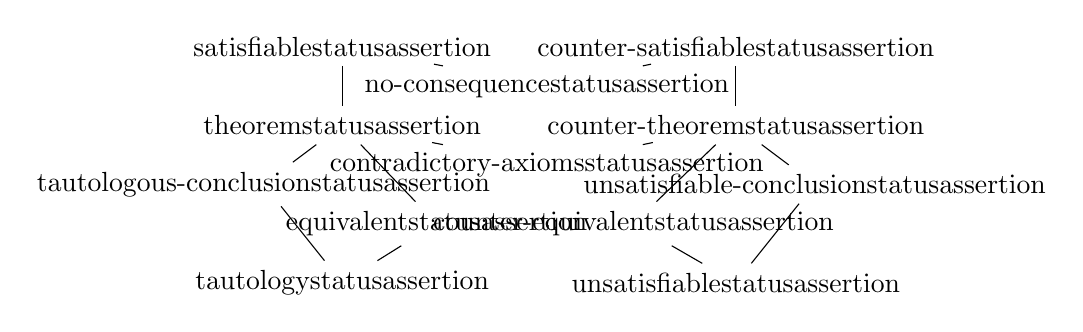
\begin{tikzpicture}
    \node (sat) at (1,4) {\attval{satisfiable}{status}{assertion}};
    \node (csat) at (6,4) {\attval{counter-satisfiable}{status}{assertion}};
    \node (thm) at (1,3) {\attval{theorem}{status}{assertion}};
    \node (cthm) at (6,3) {\attval{counter-theorem}{status}{assertion}};
    \node (tcon) at (0,2.25) {\attval{tautologous-conclusion}{status}{assertion}};
    \node (eqv) at (2.2,1.75) {\attval{equivalent}{status}{assertion}};
    \node (noc) at (3.6,3.5) {\attval{no-consequence}{status}{assertion}};
    \node (cax) at (3.6,2.5) {\attval{contradictory-axioms}{status}{assertion}};
    \node (ceqv) at (4.7,1.75) {\attval{counter-equivalent}{status}{assertion}};
    \node (ucon) at (7,2.25) {\attval{unsatisfiable-conclusion}{status}{assertion}};
    \node (taut) at (1,1) {\attval{tautology}{status}{assertion}};
    \node (usat) at (6,1) {\attval{unsatisfiable}{status}{assertion}};
    \draw (sat) -- (noc);
    \draw (sat) -- (thm);
    \draw (csat) -- (noc);
    \draw (csat) -- (cthm);
    \draw (thm) -- (tcon);
    \draw (thm) -- (cax);
    \draw (cthm) -- (cax);
    \draw (thm) -- (eqv);
    \draw (cthm) -- (ucon);
    \draw (cthm) -- (ceqv);
    \draw (tcon) -- (taut);
    \draw (eqv) -- (taut);
    \draw (ucon) -- (usat);
    \draw (ceqv) -- (usat);
  \end{tikzpicture}
\end{scriptsize}
\end{myfig}
\end{omgroup}

\begin{omgroup}[id=type-assertions]{Type Assertions}

In the last section, we have discussed the \element{type} elements in \element{symbol}
declarations. These were axiomatic (and thus {\indextoo{theory-constitutive}}) in
character, declaring a symbol to be of a certain type, which makes this information
available to type checkers that can check well-typedness (and thus plausibility) of the
represented mathematical objects.

\begin{omtext}
However, not all type information is axiomatic, it can also be deduced from other sources
knowledge. We use the same \element{type} element we have discussed in
\sref{type-axioms} for such \inlinedef{\defii{type}{assertions},
  i.e. non-constitutive statements that inform a type-checker}. In this case, the
\element{type} element can occur at top level, and even outside a \element{theory}
element (in which case they have to specify their home theory in the
\attribute{theory}{type} attribute).
\end{omtext}

{\Mylstref{term-declaration}} contains a type assertion $x+x\colon evens$, which makes the
information that doubling an integer number results in an even number available to the
reasoning process.

\begin{lstlisting}[label=lst:term-declaration,
  caption={A Term declaration in \omdoc.},
  index={type,assertion}]
<type xml:id="double-even.td" system="#POST" 
      theory="adv.int" for="plus" just-by="#double-even">
  <m:math>
    <m:apply><m:plus/>
      <m:ci type="integer">X</m:ci>
      <m:ci type="integer">X</m:ci>
    </m:apply>
  </m:math>
  <m:math>
    <m:csymbol definitionURL="http://cds.omdoc.org/integers/evens"/>
  </m:math>
</type>

<Assertion xml:id="double-even" type="lemma" theory="adv.int">
  <FMP>
    <m:math>
      <m:apply><m:forall/>
        <m:bvar><m:ci xml:id="x13" type="integer">X</m:ci></m:bvar>
        <m:apply><m:in/>
          <m:apply><m:plus/>
            <m:ci definitionURL="x13" type="integer">X</m:ci>
            <m:ci definitionURL="x13" type="integer">X</m:ci>
          </m:apply>
          <m:csymbol definitionURL="http://cds.omdoc.org/nat/evens"/>
        </m:apply>
      </m:apply>
    </m:math>
  </FMP>
</assertion>
\end{lstlisting}
The body of a type assertion contains two mathematical objects, first the type of
the object and the second one is the object that is asserted to have this
type.
\end{omgroup}

\begin{omgroup}[id=alternative]{Alternative Definitions}

  In contrast to what we have said about {\twintoo{conservative}{extension}s} at the end
  of \sref{definitions}, mathematical documents often contain multiple definitions for a
  concept or mathematical object. However, if they do, they also contain a careful
  analysis of equivalence among them. \omdoc allows us to model this by providing the
  \element{alternative} element.  Conceptually, an alternative definition or axiom is
  just a group of assertions that specify the equivalence of logical formulae. Of course,
  alternatives can only be added in a consistent way to a body of mathematical knowledge,
  if it is guaranteed that it is equivalent to the existing ones.  

\begin{definition}[id=alternative.def]
  The \attribute{for}{alternative} on the {\eldef{alternative }} points to the primary
  definition or assertion.  Therefore, \element{alternative} has the attributes
  \attribute{entails}{alternative} and \attribute{entailed-by}{alternative}, that
  specify {\element{assertion}s} that state the necessary entailments. It is an
  {\indextoo{integrity condition}} of \omdoc that any \element{alternative} element
  references at least one \element{definition} or \element{alternative} element that
  entails it and one that it is entailed by (more can be given for convenience). The
  \attribute{entails-thm}{alternative}, and \attribute{entailed-by-thm}{alternative}
  attributes specify the corresponding assertions. This way we can always reconstruct
  equivalence of all definitions for a given symbol. As alternative definitions are not
  theory-constitutive, they can appear outside a \element{theory} element as long as
  they have a \attribute{theory}{alternative} attribute.
\end{definition}
\end{omgroup}

\begin{omgroup}[short=Assertional Statements,id=assertional-statements]{Assertional Statements}

There is another distinction for statements that we will need in the following. Some kinds
of mathematical statements add information about the mathematical objects in question,
whereas other statements do not. For instance, a symbol declaration only declares an
unambiguous name for an object.
\begin{definition}[display=flow,id=assertional.def]
  We will call the following \omdoc elements
  \adefii{assertional}{assertional}{element}: \element{axiom} (it asserts central
  properties about an object), \element{type} (it asserts type properties about an
  object), \element{definition} (this asserts properties of a new object), and of course
  \element{assertion}.
\end{definition}

The following elements are considered non-assertional: \element{symbol} (only a name is
declared for an object), \element{alternative} (here the assertional content is carried
by the \element{assertion} elements referenced in the structure-carrying attributes of
\element{alternative}).  For the elements introduced below we will discuss whether they
are assertional or not in their context. In a nutshell, only statements introduced by the
module {\ADTmodule{spec}} (see \sref{adt}) will be assertional.
\end{omgroup}
\end{module}
\end{omgroup}

\begin{omgroup}[id=examples]{Mathematical Examples in OMDoc}
\begin{module}[id=examples]

In mathematical practice examples play a great role, e.g. in concept formation as
witnesses for definitions or as either supporting evidence, or as counter-examples for
conjectures.  Therefore examples are given status as primary objects in \omdoc.
Conceptually, we model an example $\cE$ as a pair $(\cW,\bA)$, where
$\cW=(\cW_1,\ldots,\cW_n)$ is an $n$-tuple of mathematical objects and $\bA$ is an
assertion. If $\cE$ is an example for a mathematical concept given as an \omdoc symbol
$\bS$, then $\bA$ must be of the form $\bS(\cW_1,\ldots,\cW_n)$.
  
If $\cE$ is an example for a conjecture $\bC$, then we have to consider the situation more
carefully. We assume that $\bC$ is of the form $\cQ\bD$ for some formula $\bD$, where
$\cQ$ is a sequence $\cQ_1W_1,\ldots,\cQ_mW_m$ of $m\geq n=\#\cW$ quantifications of using
quantifiers $\cQ_i$ like $\forall$ or $\exists$.  Now let $\cQ'$ be a sub-sequence of
$m-n$ quantifiers of $\cQ$ and $\bD'$ be $\bD$ only that all the $W_{i_j}$ such that the
$\cQ_{i_j}$ are absent from $\cQ'$ have been replaced by $\cW_j$ for $1\leq j\leq n$.  If
$\cE=(\cW,\bA)$ supports $\bC$, then $\bA=\cQ'\bD'$ and if $\cE$ is a counter-example for
$\bC$, then $\bA=\neg\cQ'\bD'$.
  
\begin{definition}[id=example.def]
  \omdoc specifies this intuition in an {\eldef{example}} element that contains
  mathematical vernacular as a \element[ns-elt=h]{p} elements for the description and
  $n$ mathematical objects (the witnesses). It has the attributes
\begin{description}
\item[\attribute{for}{example}] specifying for which concepts or assertions
    it is an example.  This is a reference to a {\indextoo{whitespace-separated
    list}} of {\indextoo{URI}} references to \element{symbol},
    \element{definition}, or \element{assertion} elements.
\item[\attribute{type}{example}] specifying the aspect, the value is one of
  \attval{for}{type}{example} or \attval{against}{type}{example}
\item[\attribute{assertion}{example}] a reference to the assertion $\bA$
  mentioned above that formally states that the witnesses really form an example for the
  concept of assertion. In many cases even the statement of this is non-trivial
  and may require a proof.
\end{description}
\end{definition}

\element{example} elements are considered
\twinalt{non-assertional}{assertional}{element} in \omdoc, since the assertional part is
carried by the \element{assertion} element referenced in the
\attribute{assertion}{example} attribute.

Note that the list of mathematical objects in an \element{example} element does not
represent multiple examples, but corresponds to the argument list of the symbol, they
exemplify. In the example below, the symbol for monoid is a three-place relation (see the
type declaration in {\mylstref{symbol}}), so we have three witnesses.

\begin{lstlisting}[label=lst:example,mathescape,
  caption={An \omdoc representation of a mathematical example},
  index={example,for,type,assertion}]
<symbol name="strings-over"/>
<definition xml:id="strings.def" for="strings-over">$\ldots$ $A^*$ $\ldots$</definition>
<symbol name="concat"/>
<definition xml:id="concat.def" for="concat">$\ldots$ $::$ $\ldots$</definition>
<symbol name="empty-string"/>
<definition xml:id="empty-string.def" for="empty-string">$\ldots$ $\epsilon$ $\ldots$</definition>
$\ldots$
<assertion xml:id="string.struct.monoid" type="lemma">
  <h:p>$(A^*,::,\epsilon)$ is a monoid.</h:p>
  <FMP>$mon(A^*,::,\epsilon)$</FMP>
</assertion>
$\ldots$
<example xml:id="mon.ex1" for="monoid" type="for"
        assertion="string.struct.monoid">
  <h:p>The set of strings with concatenation is a monoid.</h:p>
  <OMA id="nat-strings">
    <OMS cd="strings" name="strings"/>
    <OMS cd="setname1" name="N"/>
  </OMA>
  <OMS cd="strings" name="concat"/>
  <OMS cd="strings" name="empty-string"/>
</example>

<assertion xml:id="monoid.are.groups" type="false-conjecture">
 <h:p>Monoids are groups.</h:p>
 <FMP>$\allcdot{S,o,e}{mon(S,o,e)\rightarrow\excdot{i}{group(S,o,e,i)}}$</FMP>
</assertion>

<example xml:id="mon.ex2" for="#monoids.are.groups" type="against"
        assertion="strings.isnt.group">
  <h:p>The set of strings with concatenation is not a group.</h:p>
  <OMR href="#nat-strings"/>
  <OMS cd="strings" name="strings"/>
  <OMS cd="strings" name="concat"/>
  <OMS cd="strings" name="empty-string"/>
</example>

<assertion xml:id="strings.isnt.group" type="theorem">
  <h:p>$(A^*,::,\epsilon)$ is a monoid, but there is no inverse function for it.</h:p>
</assertion>
\end{lstlisting}

In {\mylstref{example}} we show an example of the usage of an \element{example} element
in \omdoc: We declare constructor symbols {\snippet{strings-over}}, that takes an
{\indextoo{alphabet}} $A$ as an argument and returns the set $A^*$ of
{\indextoo{strings}s} over $A$, {\snippet{concat}} for {\twintoo{strings}{concatenation}}
(which we will denote by $::$), and {\snippet{empty-string}} for the
{\twintoo{empty}{string}} $\epsilon$.  Then we state that $\cW=(A^*,::,\epsilon)$ is a
monoid in an \element{assertion} with {\snippet{xml:id="string.struct.monoid"}}.  The
\element{example} element with {\snippet{xml:id="mon.ex1"}} in {\mylstref{example}} is
an example for the concept of a monoid, since it encodes the pair $(\cW,\bA)$ where $\bA$
is given by reference to the assertion {\snippet{string.struct.monoid}} in the
\attribute{assertion}{example} attribute.  Example {\snippet{mon.ex2}} uses the pair
$(\cW,\bA')$ as a {\indextoo{counter-example}} to the {\twintoo{false}{conjecture}}
{\snippet{monoids.are.groups}} using the assertion {\snippet{strings.isnt.group}} for
$\bA'$.
\end{module}
\end{omgroup}

\begin{omgroup}[id=inline-statements]{Inline Statements}
\begin{module}[id=inline-statements]
 
Note that the infrastructure for statements introduced so far does its best to mark up the
interplay of formal and informal elements in mathematical documents, and make explicit the
influence of the context and their contribution to it. However, not all statements in
mathematical documents can be adequately captured directly.  Consider for instance the
following situation, which we might find in a typical mathematical textbook.
\begin{sblockquote}
  {\presbf{Theorem 3.12}}: {\presem{In a monoid $M$ the left unit and the right unit
      coincide, we call it the {\presbf{unit}} of $M$.}}
\end{sblockquote}
The overt role of this text fragment is that of a mathematical theorem --- as indicated by
the cue word ``{\presbf{Theorem}}'', therefore we would be tempted represent it as an
\element{omtext} element with the value \attval{theorem}{type}{attribute} for the
\attribute{type}{attribute} attribute. But the relative clause is clearly a
{\indextoo{definition}} (the {\indextoo{definiens}} is even marked in boldface). What we
have here is an aggregated verbalization of two mathematical statements. In a simple case
like this one, we could represent this as follows:

\begin{lstlisting}[mathescape,caption=A Simple-Minded Representation of {\presbf{Theorem 3.12}}]
<assertion type="theorem" style="display=flow">
  <h:p>In a monoid $M$, the left unit and the right unit coincide,</h:p>
</assertion>
<definition for="unit" style="display:flow">
   <h:p>we call it the <term role="definiendum" name="unit">unit</term> of $M$</h:p>
</definition>
\end{lstlisting}

But this representation remains unsatisfactory: the definition is not part of the theorem,
which would really make a difference if the theorem continued after the inline
definition. The real problem is that the inline definition is linguistically a
phrase-level construct, while the \element{omtext} element is a discourse-level
construct. However, as a phrase-level construct, the inline definition cannot really be
taken as stand-alone, but only makes sense in the context it is presented in (which is the
beauty of it; the re-use of context). With the \element[ns-elt=h]{span} element and its
\attribute[ns-elt=h]{verbalizes}{span}, we can do the following:

\begin{lstlisting}[mathescape,caption=An Inline Definition]
<assertion xml:id='unit-unique' type="theorem" >
  <h:p>In a monoid M, the left unit and the right unit coincide,
    <h:span verbalizes="#unit-def">we call it the unit of M</h:span>.</h:p>
</assertion>
<symbol name="unit"/>
<definition xml:id="unit-def" for="unit" just-by='#unit-unique'>
  <h:p>We call the (unique) element of a monoid M that acts as a left 
    and right unit the <term role="definiendum" name="unit">unit</term> of M.</h:p>
</definition>
\end{lstlisting}

thus we would have the phrase-level markup in the proper place, and we would have an
explicit version of the definition which is standalone\footnote{Purists could use the CSS
  attribute \attribute{style}{definition} on the \element{definition} element with
  value {\attvalshort{display:none}{style}} to hides it from the document; it might also
  be placed into another document altogether}, and we would have the explicit relation
that states that the inline definition is an ``abbreviation'' of the standalone
definition.\ednote{we probably also need inline examples and inline assertions, see
  \tracticket{1498}.}
\end{module}
\end{omgroup}

%%% Local Variables:
%%% mode: latex
%%% TeX-master: t
%%% End:
